\documentclass[10pt,a4paper]{report}
\usepackage[latin1]{inputenc}
\usepackage[english]{babel}
\usepackage{amsmath}
\usepackage{amsfonts}
\usepackage{amssymb}
\usepackage{graphicx}
\usepackage{hyperref}
\usepackage{float}
\author{Mounir NASR ALLAH}
\title{Storage Encryption for the Cloud - Irmin Project}


\newcommand{\HRule}{\rule{\linewidth}{0.5mm}}

\usepackage{listings}
\usepackage{xcolor}

\definecolor{grey}{rgb}{0.97,0.97,0.97}
\definecolor{white}{rgb}{1,1,1}
\definecolor{red}{rgb}{1.41,0,0}
\definecolor{green}{rgb}{0,1.41,0}
\definecolor{orange}{rgb}{0,0.23,0.6}

\lstset{
  language=[Objective]Caml,
  breaklines=true,
  extendedchars=\true,
  inputencoding=utf8,
  basicstyle=\ttfamily,
  frame=single,
  rulecolor=\color{black},
  escapechar=°,
  backgroundcolor=\color{grey},
  rulecolor=\color{white},
  keywordstyle=\color{orange},
  stringstyle=\color{green},
  commentstyle=\color{red},
  numberstyle=\color{green}
} 
 

\begin{document}
\begin{titlepage}
\begin{center}



\includegraphics[width=0.15\textwidth]{./img/university_of_cambridge.png}~\\[1cm]

\textsc{\LARGE University of Cambridge}\\[1.5cm]

\textsc{\Large Internship }\\[0.5cm]

\HRule \\[0.4cm]
{ \huge \bfseries Storage Encryption for the Cloud \ Irmin project\\[0.4cm] }

\HRule \\[1.5cm]

\noindent
\begin{minipage}{0.4\textwidth}
\begin{flushleft} \large
\emph{Author:}\\
Mounir \textsc{Nasr Allah}
\end{flushleft}
\end{minipage}%
\begin{minipage}{0.4\textwidth}
\begin{flushright} \large
\emph{Supervisor:} \\
Thomas \textsc{Gazagnaire}
\end{flushright}
\end{minipage}

\vfill

{\large \today}

\end{center}
\end{titlepage}

\tableofcontents


\chapter{Context}
This report is the result of six months of work at the Computer Laboratory of the University of Cambridge, within the OCaml Labs group. 
Supervised by Thomas Gazagnaire, this internship is about the security on Irmin, a database library, which is a part of a wide project called MirageOS. 


\chapter{Abstract}

An important part of Cloud applications is the storage layer, and especially the data security on this layer.
For such applications, user's data needs to move back and forth from the user's devices to untrusted computing nodes located in datacenters. This causes bandwidth and privacy issues. \newline

Irmin is a database library to control precisely the synchronization of data between distributed nodes, using the same design principles as distributed version control systems such as Git. The essence of a database is to store informations, so we blindly trust the databases and we assume that the data supplied by the latter respects the confidentiality, integrity, and availability. \newline

Irmin is designed to use a large variety of backends, is written in pure OCaml and does not depend on external C stubs; it aims is to run everywhere, from Linux to Xen unikernels. The user can specify the type of data stored on Irmin, and an automatic merge function.
If at least two files have the same hash value, we assumed that they have an identical content and is stored only once. 
This form of content is called addressable storage \cite{anderson}. \newline
  
Irmin is very conductive to be used for the cloud storage, and is favourable to be distributed, because this database is used like an append-only store, where data are not mutable, we can just perform adding and reading values. \newline

In the case that we can't trust on the storage service/device of this database (e.g. AWS S3), we need to encrypt data to ensure that an attacker or the cloud provider cannot read any of the stored information. 
We will therefore propose in this report, a scheme that allows us to encrypt data in the database, to cut all data on a same size chunk for a couple of reasons: the first one is for protecting against forensic  attacks, and the second one is for improving the data space.   \newline
 
We will also finish this report with the implementation of modules that we need to achieve this goal. \newline

\chapter{MirageOS and Xen}
\section{Xen}
Xen is a baremetal hypervisor(type 1), who allow us to run virtual machines, compatible with lots of operating systems. This hypervisor was developed by the Computer Laboratory of the University of Cambridge. Currently, lots of hardware architectures are supported such as IA-32, x86-64 and ARM.
Xen is based on a microkernel design, the virtual machine dom0 is the control domain and provide the drivers who needed for each others guest domains.\newline
\section{MirageOS}
MirageOS is an operating system library developed on OCaml, who give to the developer an API in order to develop an application. 
During the compilation process, we can target the system in which you want to execute this application: either under a "standard" operating system such as Linux/Unix or to create an independent and specialized operating system which we call Unikernel. 
This Unikernel, developed on OCaml, permit us to incorporate each basic layers and services needed for running the Unikernel under the Xen hypervisor, and nothing else. \newpage

Unikernels are very secure because of the OCaml compiler who verify the types and the security execution of code, are also very lightweight due to that during the compilation process only the dependencies library are linked and compiled, who minimize the code and therefore the vectors attack.\newline

We have the scheme bellow:  \newline  \newline

\begin{figure}[H]
\centerline{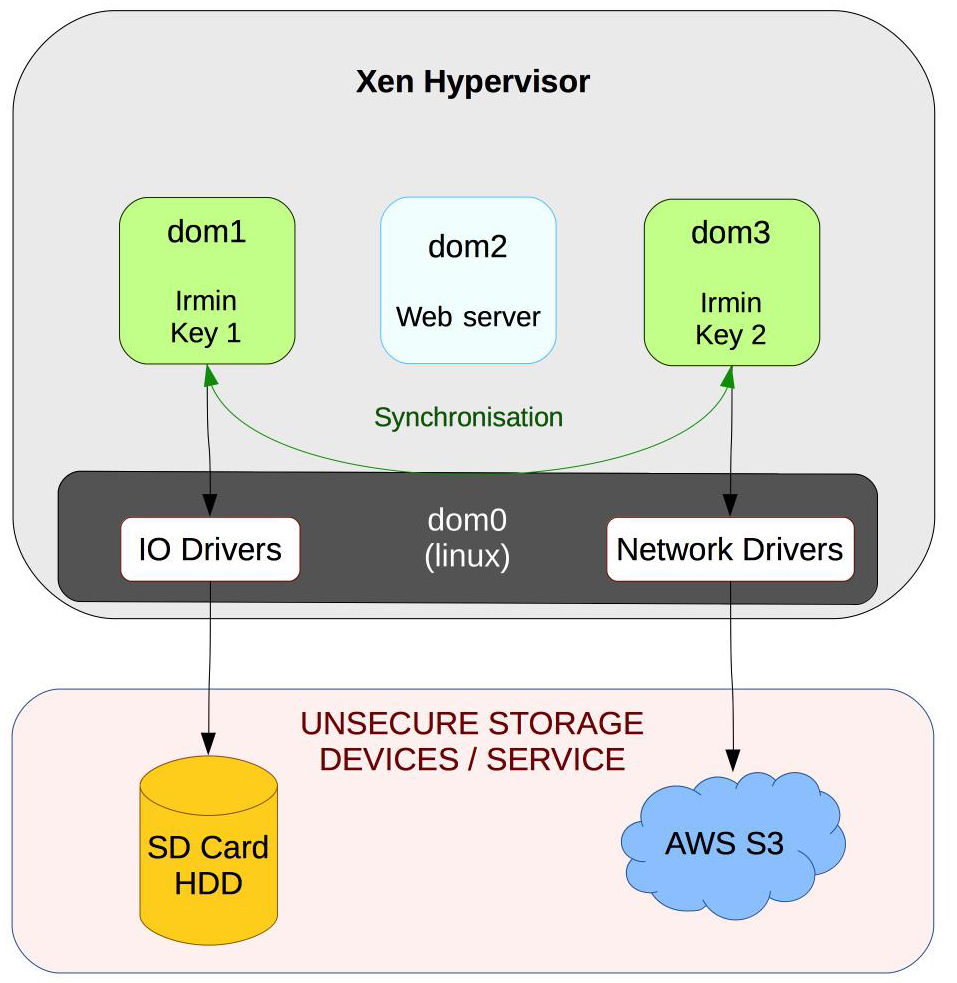
\includegraphics[scale=0.32]{img/Irmin-MirageOS.jpg}}
\caption{MirageOS VM under Xen Hypervisor}
\end{figure}

\chapter{Irmin on the context of MirageOS-Xen}

Irmin is a project which has the aim to be used on a Unikernel, and a Unikernel can be attached on a virtual disk, or can uses a service provider to store data. \newline

You cannot trust those devices or services for some reasons:
\begin{itemize}
\item If an attacker steals the login and the password of the cloud storage account, he can read data and can modify them.
\item If an attacker has access to the storage device, he can read data and can modify them.
\end{itemize}

Let's assume that we have a computer under Xen hypervisor, and we launch two unikernels running on Irmin and the other one as a web server. We can launch those virtual machines independently and attach them a storage service or device. \newline

On the context where we can create or delete unikernels on Xen, we need to set up the virtual machines with virtual devices drive, keys encryption, and some others configurations before starting the unikernel. The user can destroy and relaunch Irmin instance, the only thing needed for reusing the disk or the bucket, are the main keys and the configuration values. \newline\newline\newpage

For example, let's imagine that we develop an application like a social network, and we want to store user's picture, encrypt them for security reasons, and to profit of deduplication, because sometimes some  pictures/videos are published many times by different users.
On others words, if we have $x$ users who published the same picture, we don't want to store the same value $x$ times. \newline

\begin{figure}[H]
\centerline{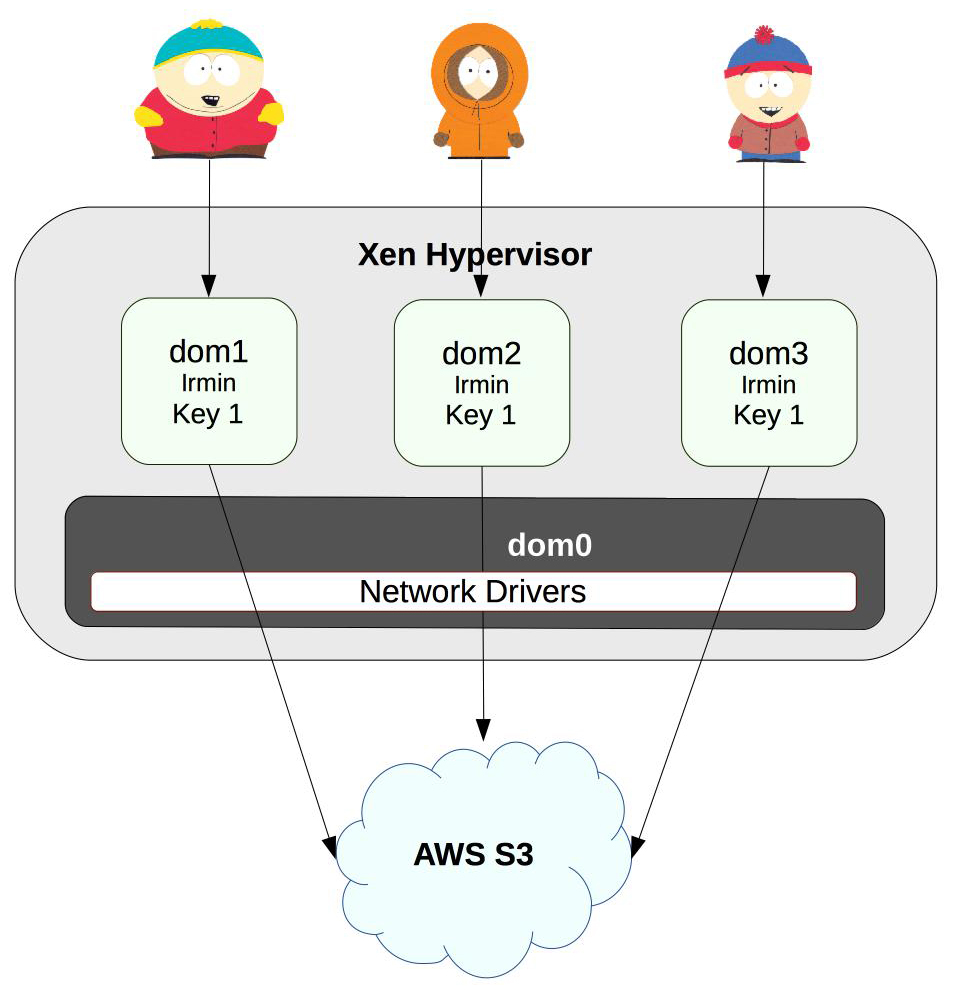
\includegraphics[scale=0.4]{img/Irmin-MirageOS-different-user-same-disk.jpg}}
\caption{Different users use the same storage layer with the same key}
\end{figure}

\newpage
Now, let's imagine that we want to develop an application where we want a strict separation between user's data, we can use different keys for each of them, the key can be derivated, or stored on a key management system.  \newline

\begin{figure}[H]
\centerline{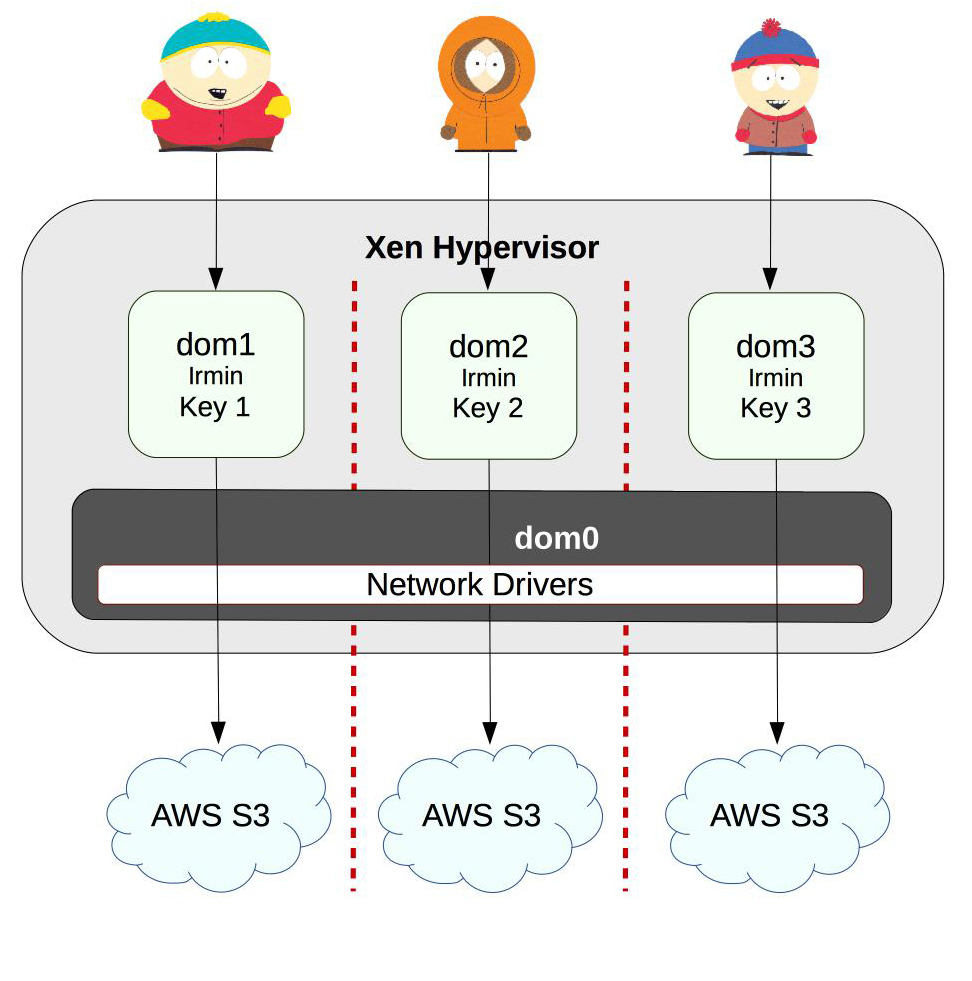
\includegraphics[scale=0.4]{img/Irmin-MirageOS-separate-user.jpg}}
\caption{Different users use different storage layers with different keys}
\end{figure}

\chapter{The essential tools}

\section{Ocaml}
OCaml is a programming language with an emphasis on expressiveness and safety. 
It includes a powerful type system, equipped with parametric polymorphism and type inference and an automatic memory management with incremental garbage collector. 
OCaml is a multi-paradigm language, is not a purely functional, it allows the use of imperative programming, it has sophisticated module system, which allows organizing modules hierarchically and parameterizing  a module and an expressive object-oriented layer. OCaml offers a compiler that produces efficient bytecode or machine code for many architectures. \newline \cite{ocaml}

Functional data structures are expected to be more flexible than their imperative counterparts. In particular, when we update an imperative data structure we typically accept that the old version of the data structure will no longer be available, but, when we update a functional data structure, we expect that both the old and new versions of the data structure will be available for further processing. A data structure that supports multiple versions is called persistent while a data structures that allows only a single version at a time is called ephemeral.
Functional programming languages have the property that all data structure are automatically persistent when imperative data structure are typically ephemeral.\newline

We say that a language element is impure if it contradicts one way or another ownership referential transparency. For example, the assignment that changes the value associated with a variable is an impure element. An impure element refers to a global or external state (e.g., a memory state) and modifies this state without this being explicit in a program (called side effect).
Some functional languages have impure elements. This is the case of OCaml.
Others are pure, that is to say completely devoid of impure element such as Haskell. Consequently, "the program using functional programming mode" does not simply mean using a functional language because it can be programmed in OCaml by adopting the imperative (using impure elements OCaml).\newline

One way to use impure element on OCaml for performing side effects, is the possibility to call C libraries from OCaml code.
This flexibility is, in fact, a very interesting feature in our case for performing encryption/decryption faster and securely. 

\section{Cstruct}

Cstruct is a library and syntax extension to make it easier to access C-like structures directly from OCaml. It supports both reading and writing to these structures, and they are accessed via the Bigarray module.\newline 

This module permits us to create, read and write buffers accessible from either OCaml code or "external" C code, on a safety way.
That also help us to manage offset, buffer overflow, etc... 
On this report, we often report to the Cstruct.t type, that simply means "a buffer".\newline

The source code of the project and the documentation are available bellows: \newline
\href{https://github.com/mirage/ocaml-cstruct}{https://github.com/mirage/ocaml-cstruct}

\section{Nocrypto}

Nocrypto is a crypto library, how allow us to use any cryptographic function with the guarantee that functions are optimized and secure.\newline

The implementation of security algorithms such as hash functions, random number generators, cipher blocks, etc... are very sensitive and needed to be implemented on low-level language programming for two-reasons: optimization (run faster) and security (try to avoid information leakages on side channels, memory leakage, etc...). \newline

It's why that nocrypto is an interface of the C implementations of cryptographic functions, that we can call on the OCaml code.

The source code of the project and the documentation are available bellows: \newline
\href{https://github.com/mirleft/ocaml-nocrypto}{https://github.com/mirleft/ocaml-nocrypto}

\section{Lwt}

Lwt is a OCaml library that provides light-weight cooperative threads. 

The source code of the project and the documentation are available bellows: \newline
\href{http://ocsigen.org/lwt/}{http://ocsigen.org/lwt/}

\chapter{Distributed Version Control}

Version control is a system that records changes to a project files, and also give you the possibility to browse across the different versions of files, revert the entire project, but also give you some information about the progression of the project and files. The naive and error prone way to have different version of a project, is to copy the directory.
Version control systems try to deal with this issue, frequently with a simple database that kept all the changes to files. \newline

\begin{figure}[H]
\centerline{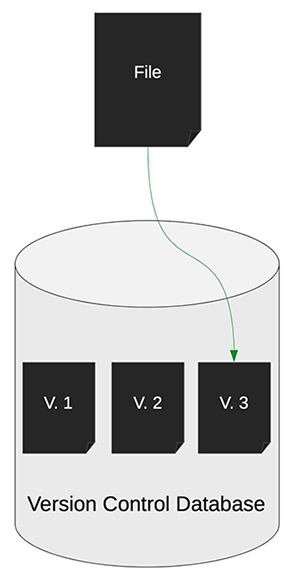
\includegraphics[scale=0.5]{img/vc.jpg}} 
\caption{Version Control}
\end{figure}

The problem is more difficult to solve when the versions of the same project are distributed on different devices.
The major issues are the classical concurrency problems, the difficulty is to merge and to synchronize the divergent versions of the project.\newline

The synchronization is when at least two nodes have different states and we try to have an identical states on every node, during this process we don't care about the content.
When we want to merge two branches of a project, we try to converge those branches, the content of the concurrent values is very important.

To deal with this problem, we have two solutions:
\begin{itemize}

\item Centralized Version Control System (CVCS): everyone knows to a certain degree what everyone else on the project is doing. Administrators have fine-grained control over who can do what.

\item Distributed Version Control System (DVCS): such as Irmin or Git, clients don't just check out the latest snapshot of the files, they fully mirror the repository. Thus, if any server dies, and these systems were collaborating via it, any of the client repositories can be copied back up to the server to restore it. Every clone is really a full backup of all the data.

\end{itemize}

After having discuss on what is a VCS, the next question is: "How we can store the modification of files on the project ?".
On VCS world, there are two main way to deal with this question. \newline

The first one, as Subversion, store an initial value of the first version of a file, and store the modifications.
On other words, if we want to go back to a specific version, we have to apply all patches (modifications) from the first version.\newline

\begin{figure}[H]
\centerline{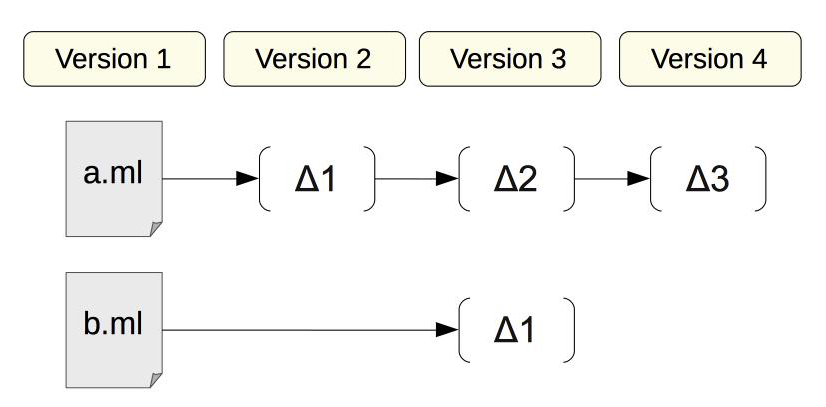
\includegraphics[scale=0.5]{img/cvs-diff.jpg}}
\caption{Modification stored as patches}
\end{figure}

The second one, such as Git and Irmin have a different approach of data versions, they store a set of snapshots. 
Every time that you modify a data and push it, they save the whole content of the file, and generate a key who is the result of a hash function (SHA-1). Then, if the files have not changed, they don't store the file again.\newline

\begin{figure}[H]
\centerline{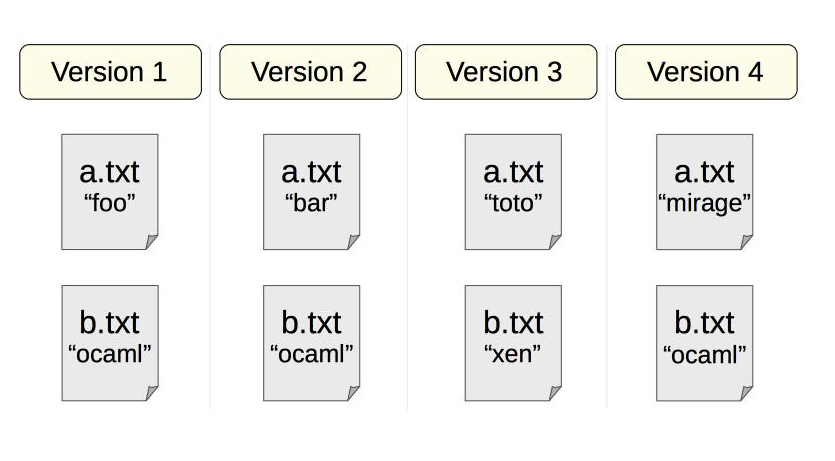
\includegraphics[scale=0.5]{img/cvs-nodiff.jpg}}
\caption{Modification stored as a new value}
\end{figure}

Those different approaches have their advantages and disadvantages, for example, to browse the history of the project, Git and Irmin simply read the history directly from your local database, almost instantly; where Subversion have to apply every patch who are performed from the initial version to the needed version. But the counterpart is that Irmin and Git need more data space for storing the different versions of the data. For trying to avoid this inconvenience, Git has a tool called "git gc" that try to safely clean-up the unnecessary files and optimize the local repository by compressing files.\newline

One of the main advantage of DVSs is that they allow us to work if we're offline, and synchronize the versions when the network connection is back.\newline

Git and Irmin have an integrity verification, everything in those DVSs is check-summed before it is stored and is then referred to by that checksum. This means it's impossible to change the contents of any file or directory without those DVSs knowing about it, and is integral to its philosophy. \newline

The mechanism that Git uses for this checksumming is called a SHA-1 hash. This is a 40-character string composed of hexadecimal characters  based on the contents of a file, example: 09cc7dfa202557a49a15ef1bff8eb8c77393b40a\newline

Irmin is quiet more flexible, the signature of the hash module is abstract, then we can choose every hash function who respect a certain signature.
Git and Irmin, have two distinct stores, the first one is an append-only store, we can only add data and you cannot erase data in any way; and a read-write store for two kinds of objects, tags who specify points in history, and branches who contains the hash of the current version of a branch.\newline

\chapter{Irmin}

\section{Introduction}
Irmin is developed on OCaml, works similarly to Git internally, and provides for the user an API to be used directly within a source code, but can also be used as a command line. 
Irmin is a Distributed Version Control, therefore we can merge data, synchronize data from others Irmin instance. \newline

One of the strengths of Irmin, is that we can customize it with some backends, we will talk about it below. 
Firstly, we need to be aware that there is a difference between mutable values (which can be changed) and immutable (which can not be changed). \newline

Internally, Irmin allows great flexibility, the user can choose any backend storage. Currently, we have a git backend, an in-memory backend, an unix backend, and a http backend.
For this, the architecture of Irmin is mainly divided into two parts, called backend stores, and which are designed to manage all operations necessary. \newline

\begin{figure}[H]
\centerline{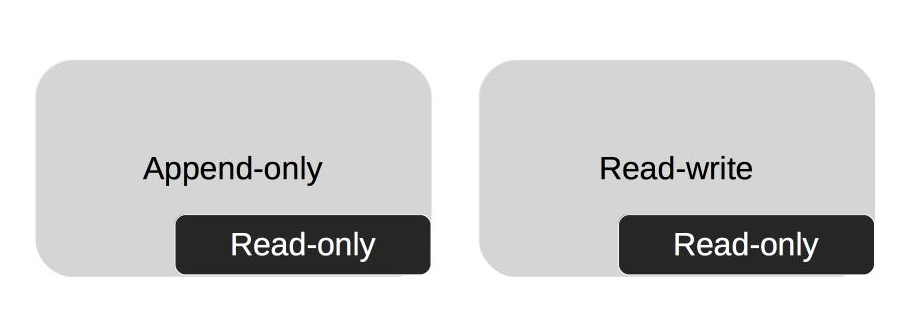
\includegraphics[scale=0.5]{img/append-only-read-write.jpg}}
\caption{Store architecture}
\end{figure}

Before developing its backends, we need to have a module called RO (Read-Only). \newline

After that, we can create two "backend stores" needed. The first one, called "append-only store" only allows to read values and to add a new values.
This store is immutable, which mean that we can not modify the values. It is extended to RO module. \newline

Then we have a second store, which allows the modification of values and is called "read-write store". 
This store is mutable, and is used for tags. It allows to link a readable strings by humans (Ir\_hum) to a key (Ir\_hash).  \newline

In the case where we use SHA-1 as cryptographic hash function, the users can send a new value to the Irmin instance and it return the hash value as a primary key.
For retrieving a value, the user has to request it by sending the hash. We have the scheme bellow: \newline

\begin{figure}[H]
\centerline{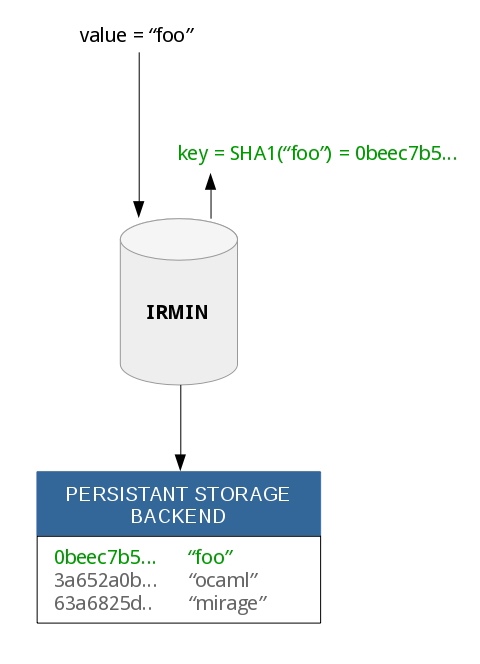
\includegraphics[scale=0.5]{img/key-value-irmin.jpg}}
\caption{Irmin philosophy}
\end{figure}

\chapter{Security}

\section{Introduction}

Cryptography is used for protecting files that we stored on disk or on an untrusted device/service by encrypted them. If the disk or the service account is stolen, files are not compromised, an attacker
can't read the content and if an attacker tries to modify the data, it will be detected during the decryption and we can handle an error and ignore the data. So we have both confidentiality and integrity for
files stored on Irmin.  \newline

In the case that we have an Irmin instance who try to communicate with the other one, we need an asymmetric encryption protocol to make sure that the data travels securely across the network, and an attacker can't eavesdrop or modify those data.\newline

In this chapter, we will not expensively talk about how a unikernel retrieve the keys, we assume that keys are retrieving during the runtime, just before that the virtual machine start, and are stored on a trust area which is dom0.\newline

Due to the fact that we cannot trust the storage layer, we need to ensure some security properties.  
\begin{itemize}
\item Confidentiality: an adversary who can read the storage layer cannot gain information about the content.
\item Data integrity: ensuring that any active attacker with access to the storage layer is unable to manipulate the contents.
\end{itemize} 

We also have some constraints given by Irmin, the ideal world corresponds to have all properties bellow:\newline

\begin{itemize}
\item  Different files and different keys producing different ciphertext
\item Same file with different keys producing different ciphertext
\item  Same file with the same key producing the same ciphertext, one of the major strength of Irmin and also Git, it's that they respect data deduplication. 
\item avoid performance decrease, we want to be able to use parallelization during the encryption, the decryption, and the storage of the data.
\item Don't control the final storage layer (mem backend, git backend, unix backend,..), so the returned key is deterministic and given by the lowest level of the storage layer. 
\item No padding because it's an attack vector
\item Each block has to be independent
\item Optimized storage consumption
\item Optimized bandwidth when synchronizing data
\item Minimum security against forensic attacks (confirmation attacks, passive localization of data...)
\end{itemize}

\section{Cryptographic hash functions}

Cryptographic hash functions are functions how take a variable length input and returns a fixed-size output. 
Hash functions are based on compression functions and have some cryptographic properties to ensure: 

\begin{itemize}
\item Pre-image resistance: given a hash value k, it should be "impossible" to find any message m such as $k=H(m)$
\item Second pre-image resistance: given a message $m_{1}$ and his resulting hash value $h_{1}$, it should  "impossible" to find an other message $m_{2}$ who we have $h_{1}=h_{2}$
\item Collision resistance: it should be impossible to find two message $m_{1}$ and $m_{2}$ such that   $h_{1} = h_{2}$
\end{itemize}

\section{Pseudorandom Generator - PRG}
Many computer applications need to create random sequences, unfortunately, the "perfect" random does not exist. 
There are many ways to create random, on some operating systems like Linux, the random generation is a function that takes several "measures" such as the CPU temperature, the memory access time, etc.\newline

It is important to have a cryptographically secure PRG , because if the random number generator is biased, then it is easy to retrieve some information, such as the key, regardless of the encryption algorithm used. Randomness plays an important role in cryptography, because the ideal model called "one-time pad" is based on precisely the perfect random generation. \newline
This cryptosystem invented around 1917 by Gilbert Vernam (1890 - 1960 ), has been proved mathematically " unbreakable " by Claude Elwood Shannon (1916 - 2001).\newline


Those PRG should ideally respect some properties:\newline
\begin{itemize}
\item Uniformity: for each generated bit , there is exactly one under two chances to get a 1 or 0 
\begin{align*}
p ( K_i = 1) = p ( K_i = 0) = \frac {1}{2}
\end{align*}
\item The independence: whatever the bits already generated for the sequence , it is impossible to predict what the next state of the bit that will be generated. 
\end{itemize}

Let's define a statistical test A that takes as input a bitstream, and simply output a boolean value that tell if the input given looks like or not looks like random.
Basically, we can construct this algorithm with the two properties mentioned early. \newline
Let $\varepsilon$ an acceptable border which ideally converge to 0.\newline
So we can have A(Input) = 1 if and only if 
\begin{align*} 
| \#1(Input) - \#0(Input) | < \varepsilon 
\end{align*}
On the ideal world, we have also: 
\begin{align*} 
p(00) = p(01) = p(10) = p(11) = \frac{1}{4} 
\end{align*}
so another statistical test must be for example:
\begin{align*} 
| \#00(Input) - (n \times \frac{1}{4} )   | < \varepsilon  
\end{align*} 

An advantage is a measure of how successfully, an attacker can be distinguishing between the PRG and a truly random generator.
Let $ G: K \rightarrow {0,1}^{n} $ be a Pseudorandom Generator, $R$ a truly random sequence, and A a statistical test on ${0,1}^{n}$.

\begin{align*} 
Adv_{PRG}[A,G] = | Pr[A(G)=1] - Pr[A(R)=1] | \in [0;1]
\end{align*} 

So when the advantage is closed to 1, that mean that G behave differently from R, and A can distinguish G from a truly random.
When is closed to 0, the G that mean that G behave similarly to R, and A cannot distinguish G from a truly random.

For make sure that a stream cipher is secure, we have to prove that the stream respects the properties, he behaves such as a truly random stream.

\section{Pseudorandom function family - PRF}

A pseudorandom function family, abbreviated PRF, as a PRG has to respect the property that no efficient algorithm can distinguish between a function chosen randomly from the PRF and a truly random function. But the difference between PRG and PRF, is that the PRG try to verify that the input is random, where PRF is about the outputs. 

\section{Block cipher - AES}
We decided to use the most knowing secure block cipher, AES.
AES is a substitution-permutation network, and is, for instance, secure because the best knowing attack has a complexity more than $2^{80}$.

\section{Operation mode - CTR}

Counter-mode encryption ("CTR mode") was introduced by Diffie and Hellman already in 1979.
CTR mode work by choosing a 128 bits random IV in the case of AES,  we start counting from this IV, and the resulting ciphertext is xored with the message.  \newline \newline
The IV doesn't need to be confidential, but the IV need to be unique, and we never have to use the same IV for encrypting two different plaintexts. During the incrementation of the IV, the counter don't have to reset to zero as well, because, in this case, we have to block encrypted with the same pad.
One thing to note is that this mode is completely paralleled. \newline


\begin{figure}[H]
\centerline{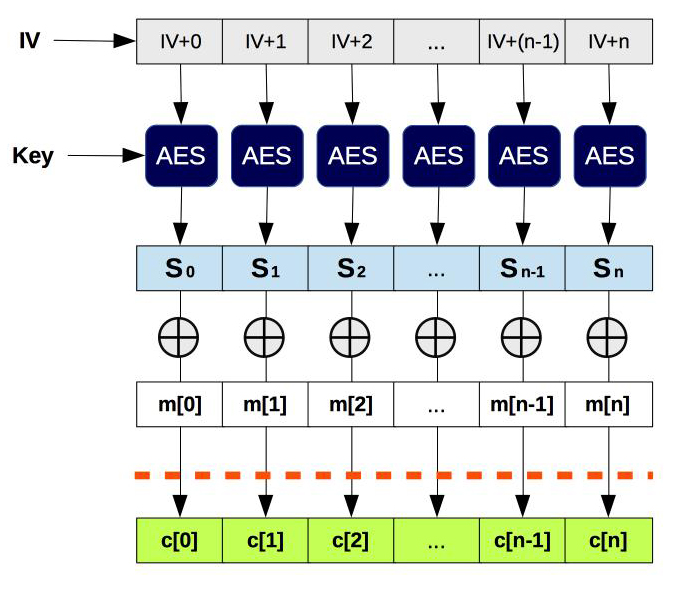
\includegraphics[scale=0.5]{img/ctr.jpg}}
\caption{Counter Mode Operation}
\end{figure}

Let F be a secure PRF $F: K \times \{0,1\}^n \rightarrow \{0,1\}^n$ \newline
Let $n$ the length of a encrypted message. We have a function who take a key, a $n$ long message, and produce a $n+1$ long ciphertext because the IV has to be included on the result. 
\begin{align*} 
E_{CTR}: K \times X^n \rightarrow X^{n+1}
\end{align*} 
Let $ |X| $ the space, $q$ the number of encrypted message with the key $K$, and $L$ the maximum length of a message. \cite{danbohen}  \newline \newline

\begin{align*} 
Adv_{CPA}[A,E_{CTR}] \le 2 \times Adv_{PRF}[B,F] + 2q^{2} \times \frac{L}{|X|}
\end{align*} 

CTR Mode is CPA secure if and only if $q^{2} \times L  << |X| $ \newline

Let's suppose that we want $ Adv_{CPA}[A,E_{CTR}] \le \frac{1}{2^{32}} $ \newline

\begin{align*}
\frac{q^{2}L}{|X|} < \frac{1}{2^{32}}
\end{align*}

Because we use AES who is a 128bits cipher block, we have: $|X| = 2^{128}$ \newline

\begin{align*}
\frac{q^{2}L}{|X|} < \frac{1}{2^{32}}
\end{align*}
\begin{align*}
\frac{q^{2}L}{2^{128}} < \frac{1}{2^{32}}
\end{align*}
\begin{align*}
q^{2}L < \frac{2^{128}}{2^{32}}
\end{align*}
\begin{align*}
q^{2}L < 2^{96}
\end{align*}
\begin{align*}
\sqrt{q^{2}L} < \sqrt{2^{96}}
\end{align*}
\begin{align*}
q\sqrt{L} < 2^{48}
\end{align*}

CTR is more secure than CBC for example, we can use the same key to encrypt more blocks than CBC could.
As well, if we have a message who his length is not a multiple of the block length, with CTR we don't need to add padding.\newline

The main issue with CTR is that it don't provide integrity and security against tampering with the cipher text. So that why we add an integrity mechanism a countermeasure against tampering.\newline

In fact, the cryptographic assumption about a block cipher's security that it is a "pseudorandom permutation" is enough but needed to prove the security of CTR, here we use AES who is currently considered as secure.\newline

 
\chapter{Chunk Module}

Irmin using deduplication strategies. So we decided to use a fixed-sized chunks for two reasons, the first one is for optimization because is we have a big file that we encrypt and an other version of this file, as we use the hash of the value for the encryption, we have a majority of space used for storing the same data on different ciphertexts; the second one is for avoid leakage about the ciphertext content (we can guess the kind of files reporting to the size). \newline
  
Thus, if at least two chunks hash have the same value, we assumed that they have an identical contents and only stored once.
This assumption permits to be sure that a key is unique. In order to split data, we need to define the structure of a chunk, and which information are necessary. \newline

We decide to implement the splitting chunk with an N-ary tree, in order to access with a constant time to a specified offset, for minimizing the number of intermediate nodes and the depth of the tree. We consider that the leaves contain data, when the nodes contain the indirections. \newline

First, we need to know what is the length of the payload (data that we have to be considered), and the second information that we needed is the kind of the chunk. We have the structure bellow:\newline

\begin{figure}[H]
\centerline{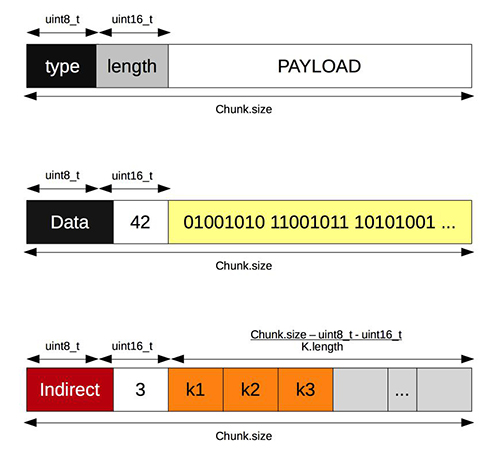
\includegraphics[scale=0.6]{img/chunk-structure.jpg}}
\caption{Chunk structure}
\end{figure}

These approaches permit us to parallelize the splitting and send all leaves without concurrency, after sending all leaves to the storage layer, we get back a list of all data chunk keys. 
Then, we construct the N-ary tree from bottom to up, the only sequential code is there, we have to wait after each level for constructing the upper level, finally we send to the upper layer the key of the root. \newline

Let's take this example: \newline
\begin{figure}[H]
\centerline{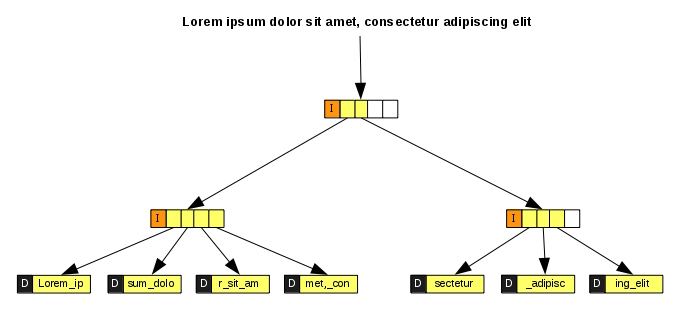
\includegraphics[scale=0.5]{img/chunk-original.jpg}}
\caption{The initial value splited}
\end{figure}

So now, if we want to add some data at the end of the initial value, we just creating the data chunks which contains the added value, and then reconstruct the right sub-tree as shown in red color. 

\begin{figure}[H]
\centerline{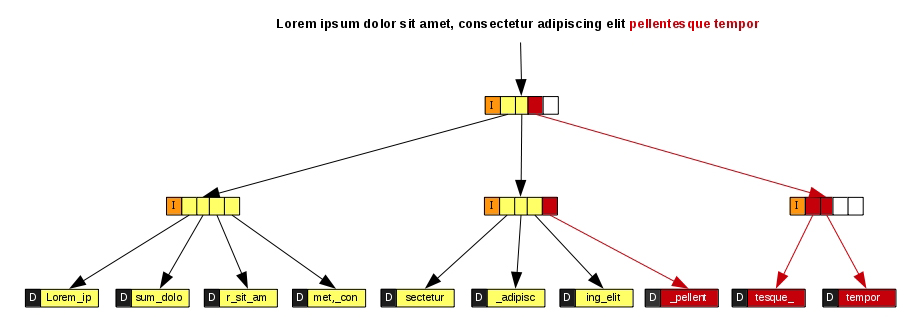
\includegraphics[scale=0.5]{img/chunk-add-at-the-end.jpg}}
\caption{Adding value at the end}
\end{figure}

When we modify some bytes of a chunk without adding more bytes, so the value length of the initial is equal to the modified one, we have the modification bellow: 

\begin{figure}[H]
\centerline{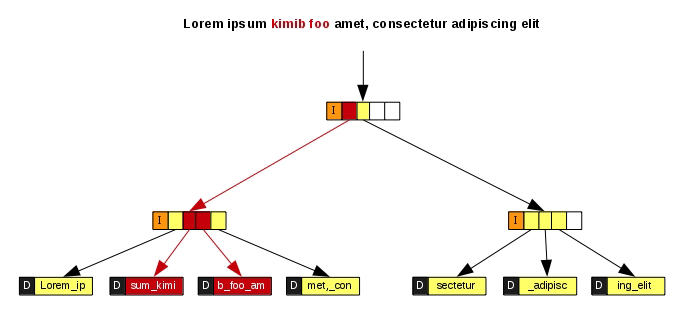
\includegraphics[scale=0.5]{img/chunk-modified-with-same-size.jpg}}
\caption{Modify some byte from the initial value}
\end{figure}

Let's consider $k$ the length of the value, $c$ the length of a chunk, and $n$ the arity of the tree \newline

\begin{itemize}
\item The number of data chunks (leaves) is: $NB_{chunks} = \frac{k}{c}$
\item The depth of the tree is equal to: $Depth = sup(\frac{log_{c}}{log_{k}})$ with the root level equal to $0$
\item The maximum number of nodes for a level i is: $NB_{chunks} = k^{i} $
\item The number of intermediate nodes for a tree with a fixed number of leaves is: $ \sum\limits_{i=1}^{Depth - 1} sup(\frac{NB_{chunks}}{n^{i}})  $
\end{itemize}

Of course, the performances of this module depends on the size of chunks. The main objective is to minimize the intermediate nodes on the tree. We have the graph bellow that give us an idea of which size to choose depend on the average size of values that we want to store. 

\begin{figure}[H]
\centerline{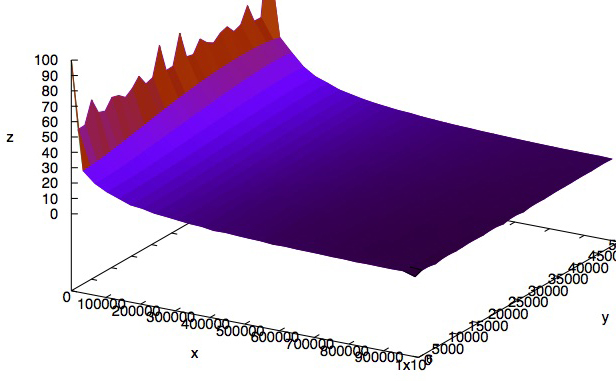
\includegraphics[scale=1]{img/chunk-graphic.jpg}}
\caption{Percentage of intermediate node depending on the size of a chunk (y) and the length value(x)}
\end{figure}

\newpage


\section{synchronization with the Chunk module}

Synchronizing means computing differences between hash sets that are stored on different nodes. With the previously schemes, we don't need to decrypt the values for computing the hash set. 
We just need to retrieve the IVs, and then send the missing chunks on the other Irmin instance. We can reconstruct the new version without decrypting or 'reading' the others chunks. \newline

\begin{figure}[H]
\centerline{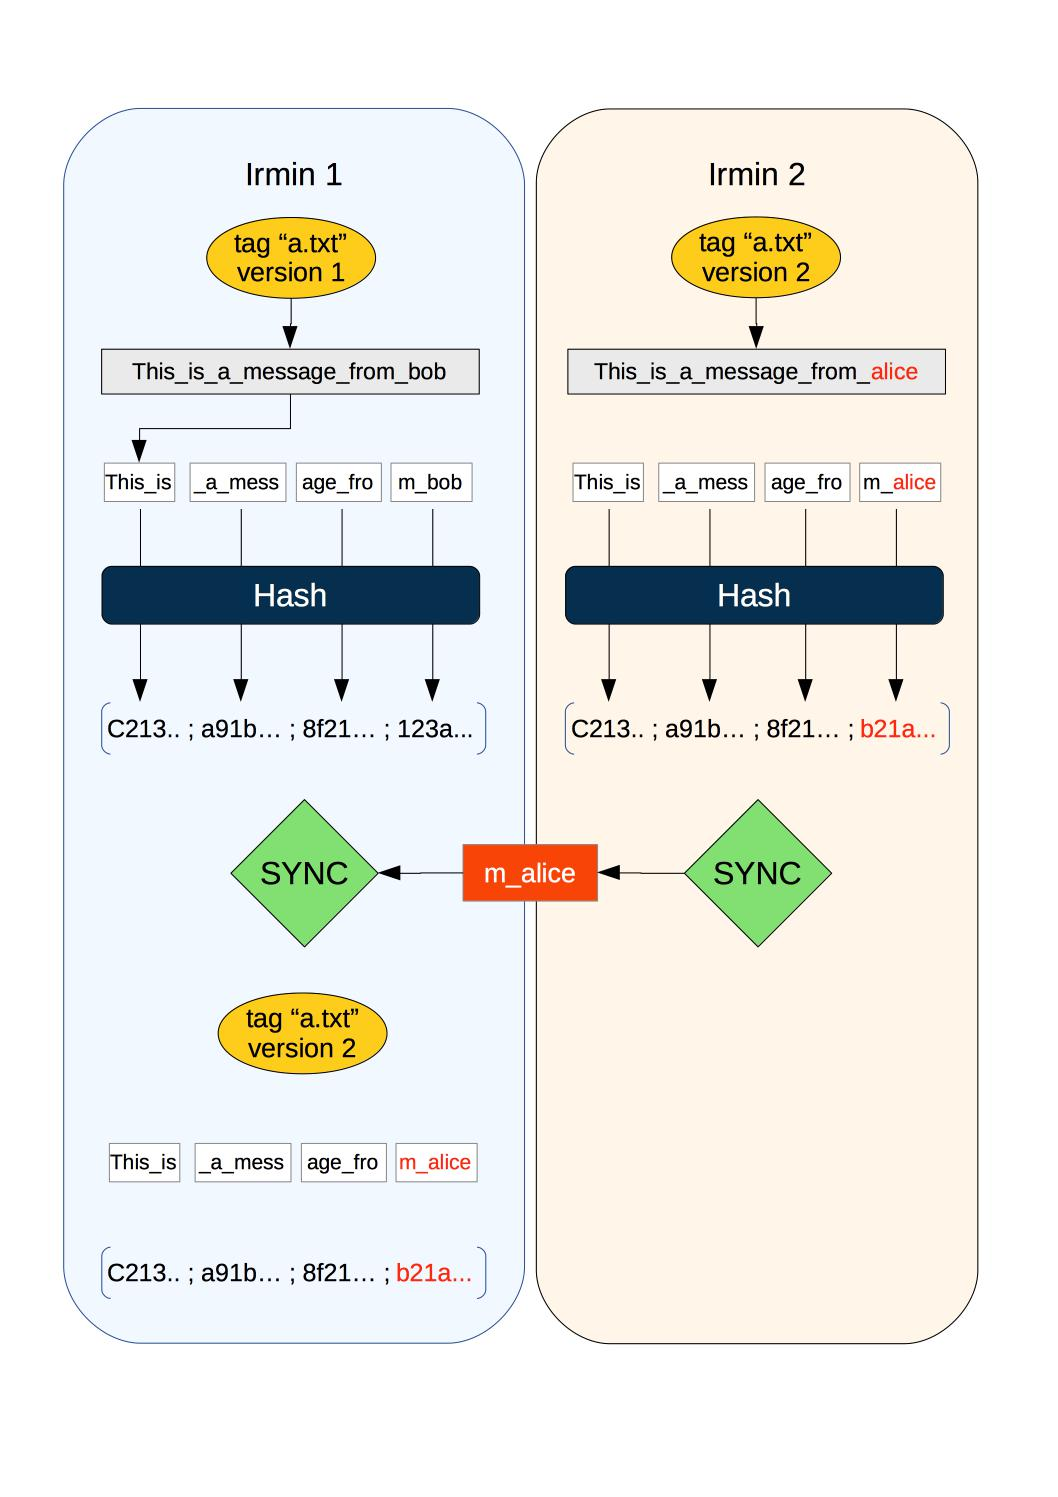
\includegraphics[scale=0.35]{img/optimization-sync-blob.jpg}}
\caption{synchronization between two Irmin instance}
\end{figure}


\chapter{Krypto Module}
Here we will outline the problematic related to data encryption in a database such as Irmin or Git. 
The solution presented below present the internal encryption of data in an instance of Irmin.
The second problem is data encryption when different instances of Irmin are communicating, but we assume that we use a library such as ocaml-TLS for securing the channel.\newline

That why the implementation of Krypto is defined by the following elements:
\begin{itemize}
\item two secret key, the first one for data encryption, and the second one for IV encryption
\item a fixed length for the data units that the key protects
\item We use AES with CTR mode.
\item The IV is the hash of the value
\item Adding an integrity mechanism, so our approach is to accompany the ciphertext by a MAC (message authentication code).
\item A countermeasure against the error propagation. If some bytes are occur in some block of ciphertext, after decryption, the error is localized to the corresponding bit of the corresponding block of plaintext. 
\end{itemize}

We illustrate the error propagation that we want to avoid bellow:\newline
Even worse than that it's actually very easy to modify ciphertext and have known effects on the corresponding plain text. This property is called malleability. If we don't trust on the device or the service storage where we send the data (e.g. a AWS S3, Dropbox, etc..), an attacker can be an active attacker and modify the ciphertext if he has the login/password of the account, or if he has a physical access of the device, and then modify data.

\newpage
Let's imagine that we have a message m, and we encrypt it using a stream cipher who give us the pad p, and the final cipher text is $m /xor p$.
Now the attacker can modify the ciphertext with a certain perturbation value a, so when we decrypt the cipher text, we have the perturbation on the resulting plain text.\newline

\begin{figure}[H]
\centerline{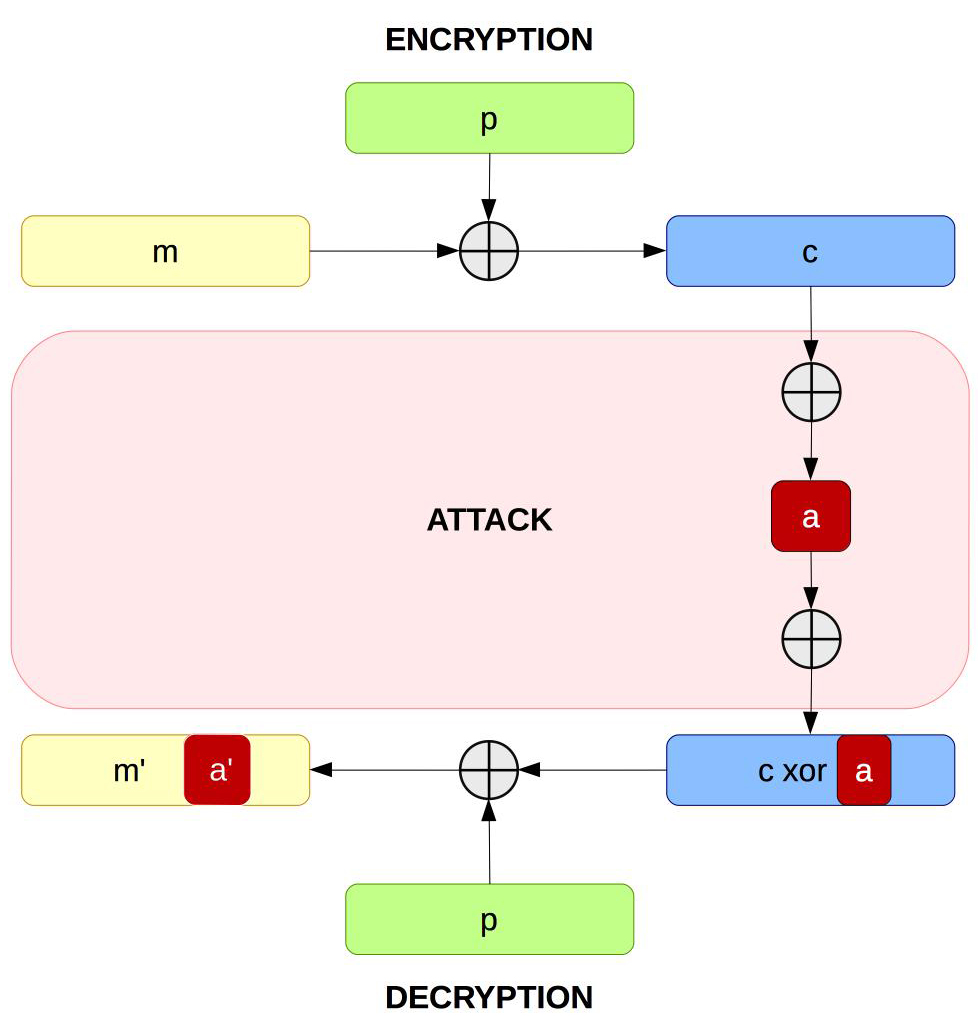
\includegraphics[scale=0.35]{img/error-propagation.jpg}}
\caption{Error propagation}
\end{figure}

\newpage

Based on AES-CTR, our solution uses a hash function H, a key data, and a deterministic IV = H(v). The solution also allows us to access to H(v) very quickly without knowing v, we can verify the Integrity,
and we have deduplication if shared keys, and no deduplication if we have different keys.\newline
The IV is encrypted as well, that permit us to be protected against confirmation attack, to solve the issue of error propagation if an attacker tries to modify the ciphertext.\newline

We have the scheme bellow:\newline

\begin{figure}[H]
\centerline{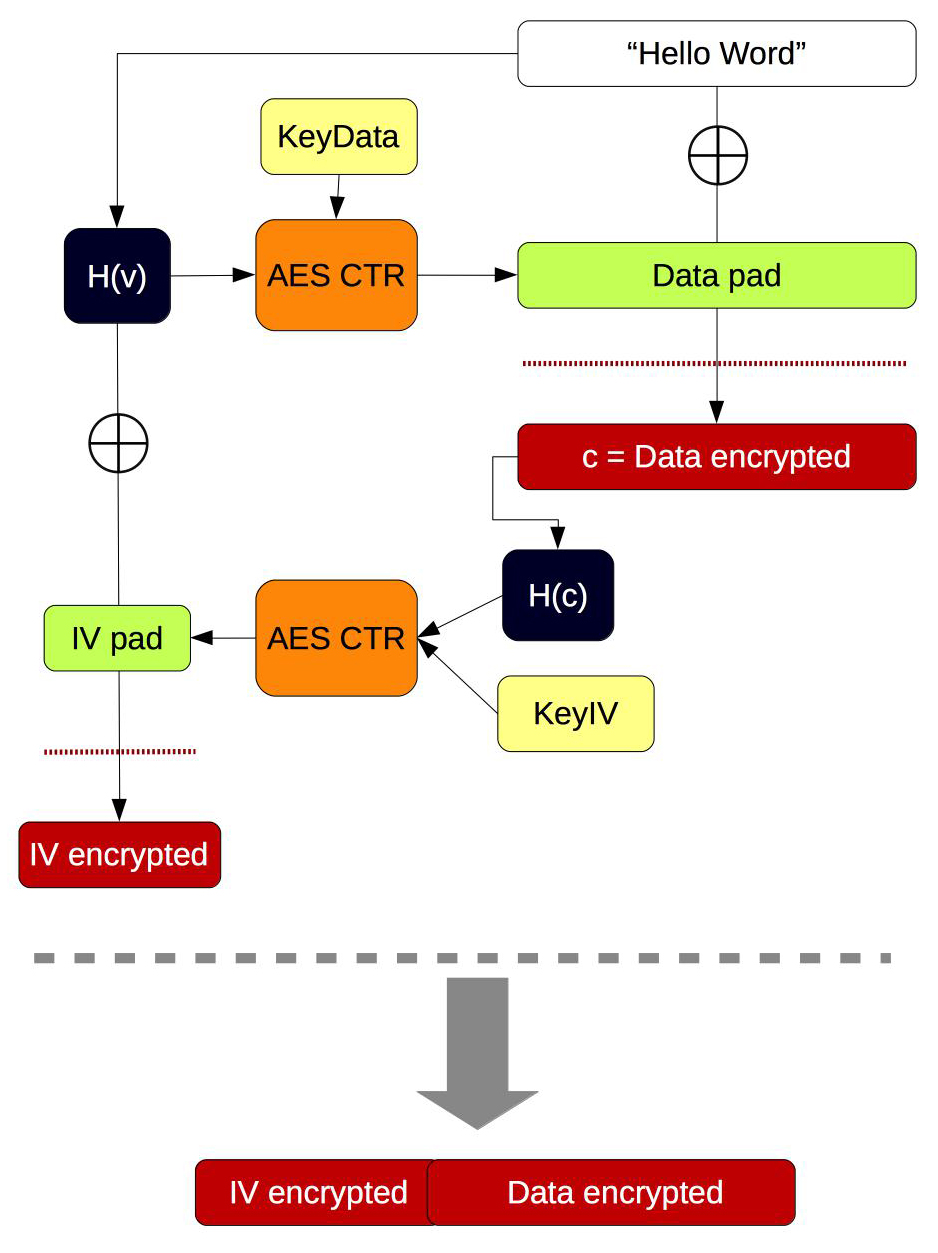
\includegraphics[scale=0.35]{img/krypto.jpg}}
\caption{Krypto scheme}
\end{figure}

\chapter{Link Module}
In the case who we use the modules Krypto and/or Chunk, we need to converge the key of the value, because internally, the key is equal to the hash of the ciphertext or to the root of the N-ary tree.
Such as Link module have to be on the top of the stack, it also includes the conversion between the type t given by the user and the Cstruct representation of the value. \newline
For example, on the scheme bellow, the instance one have the key "BOB" and the other one "ALICE". Because the keys are different, the ciphertexts are also different and we have a divergence of key that permit to access of the same value. \newline
The Link module permits to link the "public" key who is simply the hash of the value, and the internal key. For that, we store that information on a given storage backend such as the file system or the in-memory backend.\newline

\begin{figure}[H]
\centerline{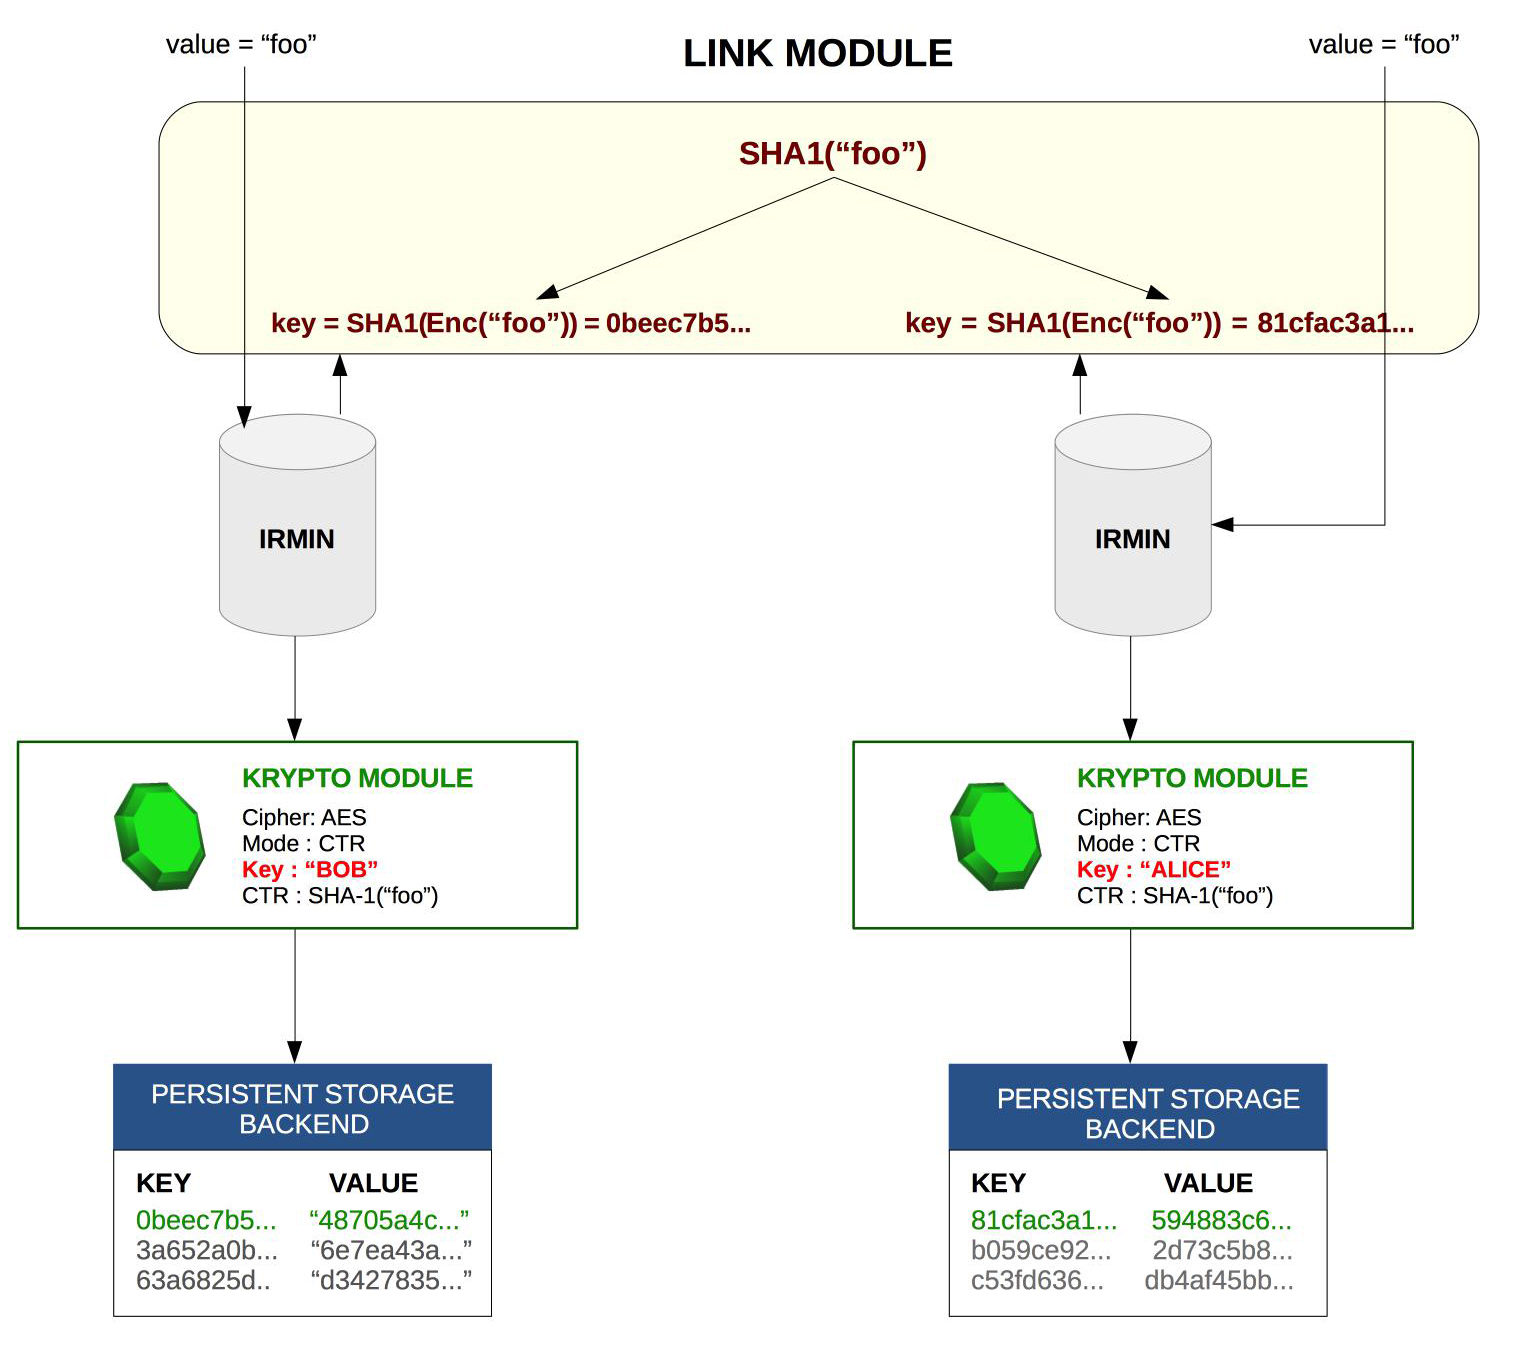
\includegraphics[scale=0.225]{img/key-value-problem-krypto-bob.jpg}}
\caption{Krypto scheme}
\end{figure}

\chapter{Conclusion}

Finally, we have three modules for resolving all problems that we had. Link module is needed if we use at least one module. 
We can use only Krypto, Chunk, or Krypto and Chunk. 
For the purpose optimizing every layer, the user have to choose the appropriate parameters such as the size of the chunks on the objective of to avoid hash collision, maximize the number of encrypted value, and to minimize the number of intermediate nodes. 

\begin{figure}[H]
\centerline{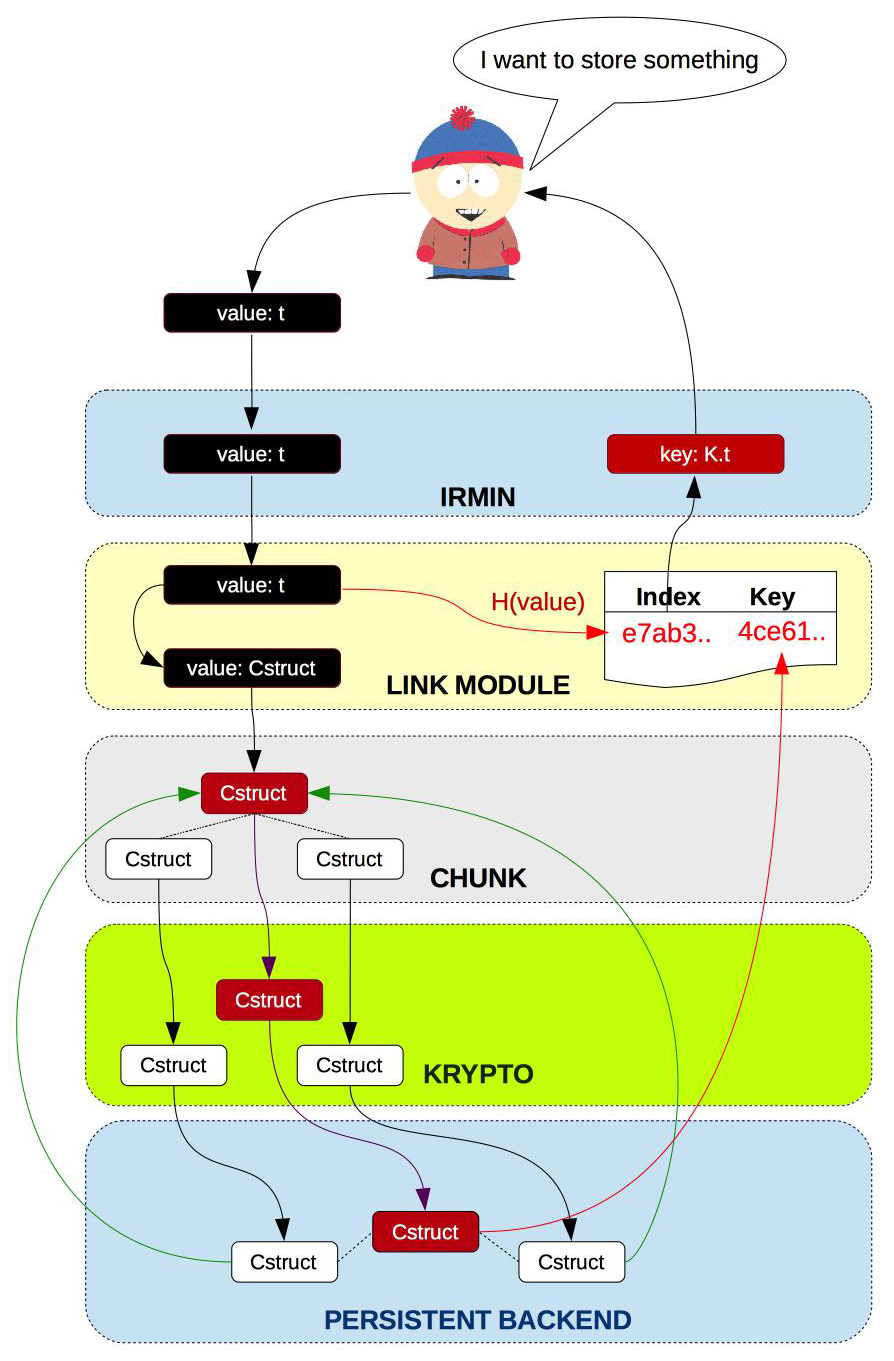
\includegraphics[scale=0.30]{img/add-krypto-chunck.jpg}}
\caption{Krypto scheme}
\end{figure}


  \begin{thebibliography}{1}

  \bibitem{anderson} Jonathan Anderson {\em Thesis: Privacy engineering for social networks} July 2002: University of Cambridge Trinity College.

  \bibitem{danbohen} Dan Boneh {\em Modes of operation: many time key (CTR)} 
  
   \bibitem{ctr} Helger Lipmaa, Phillip Rogaway, David Wagner{\em Comments to NIST concerning AES Modes of Operations: CTR-Mode Encryption} 

  \bibitem{ocaml} OCaml.org {\em https://ocaml.org} 
  
  \bibitem{mirage} MiragOS.org {\em https://mirageos.org} 
  
  \bibitem{crypto} Damien Vergnaud {\em Exercices et problemes de cryptographie} Editions Dunod

  \bibitem{uncrypto}  Paar, Christof, Pelzl, Jan {\em Understanding cryptography: a textbook for students and practitioners} Springer

  \bibitem{blockcipher} Knudsen, Lars R., Robshaw, Matthew{\em The Block Cipher Companion} Springer

  \bibitem{distrib} Jean Bacon {\em Concurrent Systems: Operating Systems, Database and Distributed Systems} Addison Wesley

  \bibitem{git} Git-scm.com {\em http://www.git-scm.com}
 
 \bibitem{unikernel} Anil Madhavapeddy, Richard Mortier, Charalampos Rotsos, David Scott, Balraj Singh, Thomas Gazagnaire, Steven Smith, Steven Hand and Jon Crowcroft {\em Unikernels: Library Operating Systems for the Cloud}



  \end{thebibliography}

\end{document}